\documentclass{article}
\usepackage[utf8]{inputenc}
\usepackage{geometry}
\usepackage{pdfpages}
\usepackage{filecontents}
\graphicspath{{images/}}
\geometry{
	a4paper,
	total={170mm,257mm},
	left=20mm,
	top=20mm,
}
\usepackage{graphicx}
\usepackage{titling}
\usepackage[american,RPvoltages]{circuiTikz}
\usepackage{tikz, tikz-cd}
\usepackage{pgfplots}
\usepackage{siunitx}
\usepackage{float}
\usepackage{enumitem}
\usepackage{amsmath,amsfonts,stmaryrd,amssymb} % Math packages
\usepackage{schemabloc}
\usepackage{tcolorbox}
\usepackage{xcolor}

\title{Amplificador Logarítmico}
\author{Rodrigo}
\date{Agosto 2024}

\usepackage{fancyhdr}
\fancypagestyle{plain}{%  the preset of fancyhdr 
	\fancyhf{} % clear all header and footer fields
	\fancyfoot[L]{\thedate}
	\fancyhead[L]{Amplificador Logarítmico}
	\fancyhead[R]{\theauthor}
}
\makeatletter
\def\@maketitle{%
	\newpage
	\null
	\vskip 1em%
	\begin{center}%
		\let \footnote \thanks
		{\LARGE \@title \par}%
		\vskip 1em%
		%{\large \@date}%
	\end{center}%
	\par
	\vskip 1em}
\makeatother

\usepackage{lipsum}  
\usepackage{cmbright}
\renewcommand{\figurename}{Figura}
%---------------------------------------------------
\tikzset{flipflop myRS/.style={flipflop,
		flipflop def={t1=R, t3=S, t6=Q, t4={\ctikztextnot{Q}}, tu={\ctikztextnot{RST}}, nu=1, n4=1 }}
}

\tikzset{flipflop myFFRS/.style={flipflop,
		flipflop def={t1=R, t3=S, t6=Q, t4={\ctikztextnot{Q}}, n4=1 }}
}
%---------------------------------------------------

\makeatletter
\newcommand*{\underarrow}{\def\@underarrow{\relax}\@ifstar{\@@underarrow}{\def\@underarrow{\hidewidth}\@@underarrow}}
\newcommand*{\@@underarrow}[2][]{\underset{\@underarrow\substack{\uparrow\if\relax\detokenize{#1}\relax\else\\#1\fi}\@underarrow}{#2}}

\newcommand*{\overarrow}{\def\@overarrow{\relax}\@ifstar{\@@overarrow}{\def\@overarrow{\hidewidth}\@@overarrow}}
\newcommand*{\@@overarrow}[2][]{\overset{\@overarrow\substack{\if\relax\detokenize{#1}\relax\else#1\\\fi\downarrow}\@overarrow}{#2}}
\makeatother

\begin{document}
	
	\maketitle
	
	\noindent\begin{tabular}{@{}ll}
		Author & \theauthor\\
	\end{tabular}
	
	\section*{Introducción}
	Los amplificadores logarítmicos y antilogarítmicos se utilizan en aplicaciones que requieren la compresión de datos de entrada analógicos, la linealización de transductores cuyas salidas son exponenciales y la multiplicación y división analógicas. A menudo se utilizan en sistemas de comunicación de alta frecuencia, incluida la fibra óptica, para peocesar señales de amplio rango dinámico.
	
	\subsection*{El logaritmo de un número}
	El logaritmo con base $b$ de un número $N$, es el exponente $a$ al cual se eleva la base $b$ para obtener el resultado o argumento $N$
	
	\begin{align}
		\log_b N = a  \Leftrightarrow N = b^a \mathrm{con} N > 0		
	\end{align}
	
	\subsection*{Logaritmos comunes o de Briggs}
	Son logaritmos cuya base es $10$, el logaritmo de cualquier número está formado por una parte que corresponde a un número entero llamado \textit{característica} y otro decimal que recibe el nombre de \textit{mantisa}. Estos logaritmos se representan de la siguiente manera:
	
	\begin{align}
		\log_{10} N = \log N
	\end{align}
	
	\begin{tcolorbox}[colback=red!5!white,colframe=red!75!black,arc=0mm,boxrule=0mm,width=(\linewidth+0.5cm),title=Propiedades de los logaritmos,colbacktitle=red!60!white,coltitle=white]
		Para cualquier $M, N, b > 0  \mathrm{ \, y \, } b \neq 0$, se cumple que
		\begin{enumerate}[] 
			\item $\log_b 1 = 0$
			\item $\log_b b = 1$
			\item $\log_b M^n = n \log_b M$
			\item $\log_b \sqrt[n]{M} = \frac{1}{n} \log_b M$
			\item $\log_b MN = \log_b M + \log_b N$
			\item $\log_b \frac{M}{N} = \log_b M - \log_b N$
			\item $\log_e M = \ln(M), \ln = \mathrm{logaritmo \,\, natural}, e =2.718 \dots$ 
		\end{enumerate}
		\rule{6cm}{0.4pt} \\
		Nota: $log_b (M +N) \neq log_b M + \log_b N$ \qquad \qquad $\log_b \left( \frac{M}{N} \right) \neq \frac{log_b M}{log_b N}$
	\end{tcolorbox}
	
	\noindent Como se mencionó anteriormente, el \textbf{logaritmico} de un número es la potencia a la cual se debe elevar la base para obtener dicho número. Un amplificador logarítmico produce una salida que es proporcional al logaritmo de la entrada y un amplificador antilogarítmico toma el antilogaritmo o el logaritmo inverso de la entrada.
	
	\section*{El amplificador logarítmico básico}
	El elemento clave en un amplificador logarítmico es un dispositivo que exhibe una característica logarítmica que, cuando se coloca en el lazo de realimentación del amplificador operacional, produce una respuesta logarítmica. Esto quiere decir que el voltaje de salida es una función del logaritmo del voltaje de entrada, como lo expresa la siguiente ecuación general:
	
	\begin{align}
		V_{out} = -K \ln (V_{in})
	\end{align}
	
	\noindent Donde $K$ es una constante y $\ln$ es el logaritmo natural en base $e$. Un \textbf{logaritmo natural} es el exponente al cual se debe elevar la base $e$ para que sea igual a una cantidad dada. Aunque se utilizarán logaritmos naturales en las fórmulas en esta sección, cada expresión puede convertirse en un logaritmo de base 10 ($\log_{10}$).
	
	\noindent La unión $pn$ de un semiconductor en la forma de diodo de unión base-emisor de un BJT proporciona una característica logarítmica. Posiblemente recuerde que un diodo tiene una característica no lineal hasta un voltaje en directa de aproximadamente $\qty{0.7}{V}$. La figura 1 muestra la curva característica, donde $V_D$ es el voltaje del diodo e $I_D$ es la corriente en el diodo en directa. 
	
	\begin{figure}[H]
		\centering	
		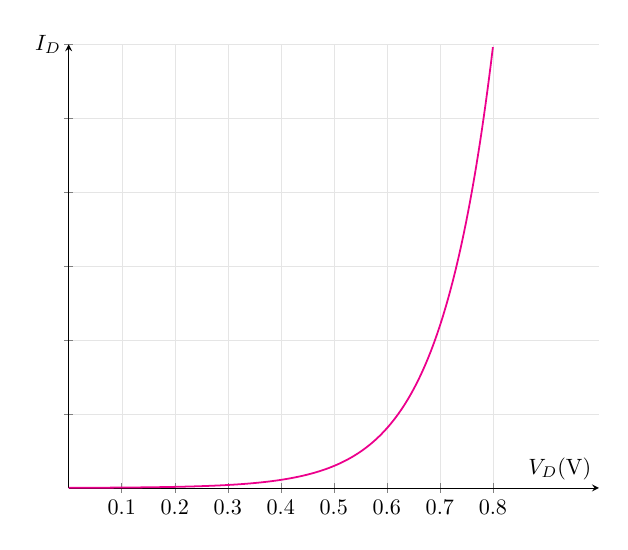
\begin{tikzpicture}[scale=0.8]
			\pgfplotsset{width=10cm,compat=1.18}			
			\begin{axis}[
				%xshift=8cm,
				%yshift=4cm,
				clip=false,
				axis y line=left,
				axis x line=middle,
				grid style={line width=.1pt, draw=gray!20},
				grid=both,
				%minor tick num=1,
				xlabel=$V_D (\mathrm{V})$,
				%ylabel=$v_s$, 
				axis y line= center,
				xmin=0,xmax=10,
				ymin=0,ymax=3,
				xtick={1,2,3,4,5,6,7,8},
				%ytick={},
				xticklabels={0.1,0.2,0.3,0.4,0.5,0.6,0.7,0.8},
				yticklabels=\empty,
				enlargelimits=false,
				]
				\addplot[smooth, magenta,thick, mark=none, domain=0:8, samples=1000] {0.001*exp(x)};
				\node[left] at(0,3){$I_D$};
			\end{axis}
		\end{tikzpicture}
		\caption{Una parte de una curva característica de un diodo}	
		\label{fig:figura1}
	\end{figure}
	

\noindent Como se puede ver en la gráfica, la cuerva del diodo no es lineal. No sólo no es lineal la curva característica, sino que es logarítmica y está especificamente definida por la siguiente fórmula:

\begin{align}
	I_D = I_S e^{\frac{V_D}{V_T}}
\end{align}	

\noindent Donde $I_S$ es la corriente de fuga en inversa y $V_T$ es una contante llamada \textbf{voltaje térmico} y está dado por

\begin{itemize}
	\item $k$ = contante de Boltzman = $8.62 \times 10^{-5} \frac{eV}{K} = 1.38 \times 10^{-23} \frac{\mathrm{joules}}{\mathrm{kelvin}}$
	\item T = temperatura absoluta en Kelvins ($K = 273.15 + \mathrm{Temperatura \, en  \, ^{\circ}C }$)
	\item q = magnitud de la carga electrónica  = $1.60 \times 10^{-19} \mathrm{coulomb}$
\end{itemize}

\noindent A una temperatura ambiente de $\qty{25}{\degreeCelsius}$ tenemos que el voltaje térmico es de 

\begin{align}
	V_T = \frac{kT}{q} = \frac{(8.62 \times 10^{-5} \mathrm{eV}/\mathrm{K})(273.15 + 25)\mathrm{K}}{1.602 \times 10^{-19} \mathrm{C}} = 160.6283 \times 10^{15} \mathrm{eV}/\mathrm{C} \nonumber
\end{align}

\noindent Recordemos que $ 1C = 6.24 \times 10^{18} e$, así

\begin{align}
	V_T = \left( 160.6283 \times 10^{15} \frac{\mathrm{eV}}{\mathrm{C}} \right) \left( \frac{\qty{1}{\coulomb}}{6.24 \times 10^{18} e} \right) \approx \qty{25.8}{\milli \volt}
\end{align}

\noindent Reescribiremos la ecuación del diodo como

\begin{align}
	I_D = I_S e^{\frac{qV_D}{kT}}
\end{align}	

\noindent Podemos determinar el voltaje en el diodo de la siguiente manera. Tomamos el logaritmo natural en ambos miembros de la ecuación (6)

\begin{align}
	\ln I_D = \ln I_S e^{\frac{qV_D}{kT}}
\end{align}

\noindent hacemos uso de las propiedades de los logaritmos para obtener

\begin{align}
	\ln I_D = \ln I_S + \ln e^{\frac{qV_D}{kT}} \nonumber \\
	\ln I_D - \ln I_S = \frac{qV_D}{kT} \nonumber \\
	\ln \frac{I_D}{IS} = \frac{qV_D}{kT} \nonumber
\end{align}

\noindent Despejando $V_D$
\begin{align}
	V_D = \left( \frac{kT}{q} \right)  \ln \left( \frac{I_D}{I_S} \right)
\end{align}

\subsection*{Amplificador logarítmico con un diodo}
Cuando se coloca un diodo en el lazo de realimentación de un circuito con amplificador operacional como se muetsra en la figura 2, se obtiene un amplificador logarítmico básico. Como la entrada inversora estpa a tierra virtual ($\qty{0}{\volt}$), la salida está a $-V_D$ cuando la entrada es positiva. Como $V_D$ es logarítmico, también lo es $V_{out}$. La salida está limitada a un valor máximo de aproximadamente $-\qty{0.7}{\volt}$ porque la característica logarítmica del diodo está restringida a voltajes por debajo de $\qty{0.7}{\volt}$. Además, la entrada debe ser positiva cuando el diodo se conecta en la dirección mostrada en la figura. Para manejar entradas negativas, se debe invertir la posición del diodo.

\begin{figure}[H]
	\centering	
	\begin{tikzpicture}[scale=0.8]
		\def\x{2.1*pi}% scalebar-x at golden ratio of x=1728px
		\def\y{320}% scalebar-y at 90% of height of y=356px
		\ctikzset{bipoles/thickness=4}
		\ctikzset{monopoles/vcc/arrow={Stealth[width=6pt,length=9pt]}}
		\ctikzset{monopoles/vee/arrow={Stealth[width=6pt,length=9pt]}}
		\draw (0,0) node[op amp, anchor=+](OA){};
		\draw (OA.-) to[short] ++(-1,0)
		to[short, -*] ++(0,2) coordinate (p1);
		\draw (p1) to[D*, f=$I_D$, v=$V_D$]  (p1 -| OA.out) to[short, -*] (OA.out);
		\draw (OA.out) to[short, -o] ++(0.5,0) node[right]{$V_O$};
		\draw (p1) to[short] ++(-1,0) coordinate (p2);
		\draw(p2) to[R, -o, l=$R_1$, f<_=$I_{in}$] ++ (-3,0) node[left]{$V_{in}$};
		\draw (OA.+) to[short] ++(-1,0) to[short] ++(0,-1) node[ground]{};
		\node[above] at (p1){$v^-$};
	\end{tikzpicture}
	\caption{Un amplificador logarítmico básico que utiliza un diodo como elemento de realimentación.}	
	\label{fig:figura2}
\end{figure}

\noindent Un análisis del circuito de la figura 2 comienza por porsiderar emplear la LCK sobre el nodo denominado $v^-$, es decir:

\begin{align}
	I_{in} &= I_D \nonumber \\
	\frac{V_{in} - v^{-}}{R_1} &= I_S e^{\frac{qV_D}{kT}} = I_S e^{\frac{q(V^{-} - V_O)}{kT}} \nonumber \\
	\frac{V_{in}}{R_1} &= I_S e^{-\frac{qV_O}{kT}} \nonumber \\
	\ln \frac{V_{in}}{R_1I_S} &= -\frac{qV_O}{kT} \nonumber
\end{align}

\noindent Al despejar para $V_O$ obtenemos

\begin{align}
	V_O = - \left( \frac{kT}{q} \right) \ln \left( \frac{V_{in}}{R_1I_S} \right) 
\end{align}

\noindent De acuerdo con la ecuación (9), el voltaje de salida es el negativo de una función logarítmica del voltaje de entrada. El valor del voltaje de eentrada y el valor del resistor $R_1$ controlan el valor de la salida. El otro factor, $I_S$ es una constante para un diodo dado.

\subsection*{Cambios de base}
Es posible hacer un cambio de base en la ecuación (9) para expresarla como un logaritmo común o de Briggs o de base 10, en lugar de un logaritmo natural, para realizar el cambio de base, utilizamos la siguiente ecuación

\begin{align}
	\log_b N = \frac{\log_a N}{\log_a b}
\end{align}

\noindent Donde

\begin{align}
	b &= e \nonumber \\
	N &= \frac{V_{in}}{R_1I_S} \nonumber \\
	a &= 10 \nonumber
\end{align}

\noindent Así

\begin{align}
	\log_e \left( \frac{V_{in}}{R_1I_S} \right) = \frac{ \log_{10} \left( \frac{V_{in}}{R_1I_S} \right) }{\log_{10} e} = \frac{ \log_{10} \left( \frac{V_{in}}{R_1I_S} \right) }{0.4343} \approx 2.30 \log_{10} \left( \frac{V_{in}}{R_1I_S} \right)
\end{align}

\noindent Por lo tanto, el voltaje de salida para el amplificador logarítmico con diodo de la figura 2 puede escribirse como

\begin{align}
	V_O = -2.30\left( \frac{kT}{q} \right) \log_{10} \left( \frac{V_{in}}{R_1I_S} \right)
\end{align}

\noindent Si asumimos una temperatura ambiente de $\qty{25}{\degreeCelsius}$ como lo hicimos en (5), el voltaje de salida puede escribirse una vez más como

\begin{align}
	V_O = -0.05934 \log_{10} \left( \frac{V_{in}}{R_1I_S} \right)
\end{align}

Es importante notar que muchos de los conceptos familiares de los circuitos lineales son irrelevantes en los amplificadores logaritmicos. Por ejemplo, la ganancia incremental de un amplificador logarítmico tiende a infinito conforme  la entrada tienda a cero, y un cambio en el offset en la salida del amplificador logarítmico es equivalente a un cambio de amplitud en su entrada 

\subsection*{Amplificador logarítmico con un BJT}
La unión base emisor de un tarnsistor de unión bipolar presenta el mismo tipo de característica logarítmica que un diodo porque también está formado por una unión $pn$, La figura 3 muestra un amplificador logarítmico con un BJT conectado en base común con el lazo de realimentación. Observe que $V_o$ con respecto a tierra es igual a $-V_{BE}$.

\begin{figure}[H]
	\centering	
	\begin{tikzpicture}[scale=0.8]
		\def\x{2.1*pi}% scalebar-x at golden ratio of x=1728px
		\def\y{320}% scalebar-y at 90% of height of y=356px
		\ctikzset{bipoles/thickness=4}
		\ctikzset{monopoles/vcc/arrow={Stealth[width=6pt,length=9pt]}}
		\ctikzset{monopoles/vee/arrow={Stealth[width=6pt,length=9pt]}}
		\draw (0,0) node[op amp, anchor=+](OA){};
		\draw (OA.-) to[short] ++(-1,0)
		to[short, -*] ++(0,3) coordinate (p1);
		\draw (p1) to[short, f=$I_C$] ++(1,0) coordinate (p3) node[npn, anchor=C,rotate=90](Q){};
		\draw (Q.E) to[short]  (p1 -| OA.out) to[short, -*] (OA.out);
		\draw (Q.B) node[ground]{};
		\draw (OA.out) to[short, -o] ++(0.5,0) node[right]{$V_O$};
		\draw (p1) to[short] ++(-1,0) coordinate (p2);
		\draw(p2) to[R, -o, l=$R_1$, f<_=$I_{in}$] ++ (-3,0) node[left]{$V_{in}$};
		\draw (OA.+) to[short] ++(-1,0) to[short] ++(0,-1) node[ground]{};
		%\node[above] at (p1){$v^-$};
		\node[right] at (Q.B){\small$+$};
		\node[right, below ] at (Q.E){\small$-$};
		\node[right=7mm, above ] at (Q.B){\small$V_{BE}$};
	\end{tikzpicture}
	\caption{Un amplificador logarítmico básico que utiliza un diodo como elemento de realimentación.}	
	\label{fig:figura3}
\end{figure}

\noindent La corriente de colector es transportada por los electrones que alcanzan la región de colector. Su dirección será opuesta a la del flujo de electrones, entrando por lo tanto a la terminal del colector. Su magnitud será porporcional a $e^{v_{BE}/V_T}$, así

\begin{align}
	I_C = I_S e^{\frac{v_{BE}}{V_T}}
\end{align}
\noindent Donde la constante de proporcionalidad $I_S$, como en el caso del diodo, es llamado \textbf{corriente de saturación} y es un parámetro del transistor.

\noindent Conociendo la ecuación para la corriente del colector, procedemos a atilizar la LCK sobre el nodo de la entrada inversara, con lo cual obtenemos:

\begin{align}
	I_{in} &= I_C \nonumber \\
	\frac{V_{in}}{R_1} &= I_S e^{\frac{v_{BE}}{V_T}} \nonumber \\
	\frac{V_{in}}{R_1I_S} &= e^{\frac{v_{BE}}{V_T}} \nonumber \\
	\ln \left( \frac{V_{in}}{R_1I_S} \right) &= \ln e^{\frac{v_{BE}}{V_T}} \nonumber \\
	\ln \left( \frac{V_{in}}{R_1I_S} \right) &= \frac{v_{BE}}{V_T} = -\frac{V_O}{V_T}  \nonumber
\end{align}

\noindent La expresión para el voltaje de salida es:

\begin{align}
	V_O = -V_T \ln \left( \frac{V_{in}}{R_1I_S} \right) = -\left( \frac{kT}{q} \right) \ln \left( \frac{V_{in}}{R_1I_S} \right)
\end{align}

\noindent Notamos que la ecuación expresada en (15) en básicamente la misma que en (9), por lo que es posible expresarla en términos de logaritmo en base 10 dando como resultado el mismo que en la ecuación (13).

\noindent Estos tipos de amplificadores logarítmicos  tienen tres principales desventajas: (1) tanto la pendiente como la intercepción son altamente dependientes de la temperatura; (2) sólo manejan señales unipolares; y (3) el ancho de banda en ambos circuitos es limitado y dependiente de la señal de amplitud de entrada. \\

\noindent A continuación, se presentarán un par de amplificadores logarítmicos más sofisticados mediante la interconexión de dos o más OpAmps que permiten una salida logarítmica en base 10 con una constante proprocional unitaria

\section*{Amplificador logarítmico 1}
En el circuito de la siguiente figura, asuma que $Q_1$ y $Q_2$ son idénticos, encuentre el valor de $R_3$ y $R_4$ de tal manera que el voltaje de salida esté dado por 

\begin{align}
	1.0 \log_{10} \left( \frac{V_2 R_1}{V_1 R_2} \right)
\end{align}

\begin{figure}[H]
	\centering	
	\begin{tikzpicture}[scale=0.8]
		\def\x{2.1*pi}% scalebar-x at golden ratio of x=1728px
		\def\y{320}% scalebar-y at 90% of height of y=356px
		\ctikzset{bipoles/thickness=4}
		\ctikzset{monopoles/vcc/arrow={Stealth[width=6pt,length=9pt]}}
		\ctikzset{monopoles/vee/arrow={Stealth[width=6pt,length=9pt]}}
		\draw (0,0) node[op amp, anchor=+](OA){};
		\draw (OA.-) to[short] ++(-1,0)
		to[short, -*] ++(0,3) coordinate (p1);
		\draw (p1) to[short] ++(1,0) coordinate (p3) node[npn, anchor=C,rotate=90](Q){};
		\draw (Q.E) to[short]  (p1 -| OA.out) to[short, -*] (OA.out);
		\draw (Q.B) node[ground]{};
		\draw (OA.out) to[short, -o] ++(0.5,0) coordinate (ao 1) node[right]{$V_{O_1}$};	
		\draw (p1) to[short] ++(-1,0) coordinate (p2);
		\draw(p2) to[R, -o, l=$R_1$] ++ (-3,0) node[left]{$V_1$};
		\draw (OA.+) to[short] ++(-1,0) to[short] ++(0,-1) node[ground]{};
		%\node[above] at (p1){$v^-$};
		\node[right] at (Q.B){\small$+$};
		\node[right, below ] at (Q.E){\small$-$};
		\node[right=7mm, above ] at (Q.B){\small$V_{BE}$};
		\draw (ao 1)++(3,0)  node[op amp, noinv input up, anchor=out, rotate=180](OA2){};
		\draw (OA2.-) to[short] ++(1,0)
		to[short] ++(0,3) coordinate (p5) to[short] ++(-1,0) coordinate (p6) node[npn, anchor=C,rotate=-90, xscale=-1](Q2){};
		\draw (Q2.B) node[ground]{};
	    \draw (Q2.E) to[short]  (p6 -| OA2.out) to[short, -*] (OA2.out);
	    \draw (OA2.out) to[short, -o] ++(-0.5,0) node[left]{$V_{O_2}$};
	    \draw (p5) to[R,*-o, l=$R_2$] ++(3,0) node[right]{$V_2$};
	    \node[left] at (Q2.B){\small$+$};
	    \node[right, below ] at (Q2.E){\small$-$};
	    \node[left=7mm, above ] at (Q2.B){\small$V_{BE}$};
	    \node[, left=8mm,above] at (Q.E){$Q_1$};
	    \node[, right=8mm,above] at (Q2.E){$Q_2$};
	    \draw (OA2.+) to[short] ++(1,0) to[short] ++(0,-1) node[ground]{};
	    \draw (OA.out) to[short] ++(0,-5) coordinate (p9);
	    \draw (OA2.out) to[short] ++(0,-6) to[R, l=$R_3$] ++(3,0) coordinate (p7) to[short] ++(1,0) node[op amp, anchor=-](OA3){};
	    \draw (p7) to[short, *-] ++(0,2) coordinate (p8);
	    \draw (p8) to[R, l=$R_4$] (p8 -| OA3.out) to[short] (OA3.out) to[short, *-o] ++(0.5,0) node[right]{$V_o$};
	    \draw (OA3.+) to[short] ++(-1,0) coordinate(p10) to[R, l=$R_3$] ++(-3,0) coordinate (p11);
	    \draw (p11) to[short] (p11 -| p9) to[short] (p9);
	    \draw (p10) to[R, l=$R_4$, *-] ++(0,-3) node[ground]{};
	\end{tikzpicture}
	\caption{Un amplificador logarítmico}	
	\label{fig:figura4}
\end{figure}

\noindent El circuito de la figura 4 está compuesto por dos amplificadores logarítmicos y un amplificador diferencial. Ya hemos encontrado el voltaje de salida para el amplificador logarítmico el cual se expuso en la ecuación (15), es decir

\begin{align}
	V_{o_1} =  -V_T \ln \left( \frac{V_1}{R_1I_S} \right) \\
	V_{o_2} =  -V_T \ln \left( \frac{V_2}{R_2I_S} \right)
\end{align}

En cuanto al amplificador diferencial tenemos que:

\begin{align}
	V_o = \frac{R_4}{R_3} \left( V_{O_2} - V_{O_1} \right)
\end{align}

\noindent Al sustituir las ecuaciones (17) y (18) en (19) obtenemos

\begin{align}
		V_o &= \frac{R_4}{R_3} \left[  -V_T \ln \left( \frac{V_1}{R_1I_S} \right) + V_T \ln \left( \frac{V_2}{R_2I_S} \right) \right] \nonumber \\ 
		&= \frac{R_4}{R_3} \left[ -V_T (\ln V_1 - \ln R_1 I_S) + V_T (\ln V_2 - \ln R_2I_S) \right] \nonumber \\
		&= \frac{R_4}{R_3} \left[ -V_T\ln V_1 + V_T \ln R_1 I_S) + V_T \ln V_2 - V_T \ln R_2I_S \right] \nonumber \\
		&= V_T\frac{R_4}{R_3} \left[ \ln V_2 - \ln V_1 + \ln R_1IS_ - \ln R_2I_S \right] \nonumber \\
		&= V_T\frac{R_4}{R_3} \ln \left( \frac{V_2I_SR_1}{V_1I_SR_2} \right)
\end{align}

\noindent Por lo tanto, el voltaje de salida está dado por:

\begin{align}
	V_T = V_T \frac{R_4}{R_3} \ln \left( \frac{V_2R_1}{V_1R_2} \right)
\end{align}

\noindent Donde $V_T \approx \qty{25.8}{\milli \volt}$ a $T = \qty{300}{\kelvin}$, así

\begin{align}
	V_o = 0.0258 \frac{R_4}{R_3} \ln \left( \frac{V_2R_1}{V_1R_2} \right)
\end{align}

\noindent Utilizamos la ecuación (10) para cambiar la base a logaritmo base 10, donde:

\begin{align}
	b = e \nonumber \\
	N =  \frac{V_2R_1}{V_1R_2} \nonumber \\
	a = 10
\end{align}

\noindent Así

\begin{align}
	\log_e \left( \frac{V_2R_1}{V_1R_2} \right) = \frac{ \log_{10} \left( \frac{V_2R_1}{V_1R_2} \right) }{\log_{10} e} = \frac{ \log_{10} \left( \frac{V_2R_1}{V_1R_2} \right) }{0.4343} \approx 2.30 \log_{10} \left( \frac{V_2R_1}{V_1R_2} \right) 
\end{align}

\noindent Al multiplicar (24) por el voltaje término tenemos que
\begin{align}
	V_o = 0.0594 \frac{R_4}{R_3} \log_{10} \left( \frac{V_2R_1}{V_1R_2} \right) 
\end{align}

\noindent Para que la ganancia dada en (25) sea iguala 1, debemos igualar las constantes multiplicativas a 1, es decir:

\begin{align}
	0.0594 \frac{R_4}{R_3} = 1\nonumber
\end{align}

\noindent El despeje de $R_4$ da como resultado

\begin{align}
	\frac{R_4}{R_3} &= \frac{1}{0.0594} = 16.8350 \nonumber \\
	R_4 &= 16.8350R_3 \nonumber
\end{align}

\noindent Si 

\end{document}